\documentclass[../../../main.tex]{subfiles}
\begin{document}
Lorsque l'étudiant sortant de classes préparatoires arrive en école d'ingénieur, l'habitude lui est venu de se gaver de connaissances toutes prêtes dans de jolis plats de porcelaine juste faces à lui. La marche est grande, et c'est peu de le dire, lorsque le même étudiant ne voit plus cette connaissance prête à être mangée face à lui, et doit aller la chercher dans le placard plus loin et parfois doit même se mettre lui-même aux fourneaux pour construire des connaissances solides à partir de sources vagues et brumeuses.

Pourtant, le métier d'ingénieur requiert cette compétence de recherche. Il ne s'agit généralement pas d'inventer comme le ferait un chercheur mais \textit{a minima} de trouver, sur Internet ou dans des livres physiques, des bouts de connaissances qu'il faut réassembler pour résoudre un problème donné. Cette nécessité ne sert évidemment pas d'excuse aux pseudo-professeurs d'écoles d'ingénieurs qui se font le plaisir de cours fumeux absents de rigueur, de pédagogie et dans le pire des cas de tout contenu digne d'intérêt académique ou industriel\footnote{Mais chuuuuut !}. Il serait d'ailleurs bien plus avantageux d'apprendre aux élèves ingénieurs cette compétence de recherche, en leurs apportant les méthodes et principes permettant de trouver les informations nécessaire à la résolution d'un problème. Il peut s'agir par exemple :
\begin{itemize}
	\item de connaître les sites web considérés comme des sources valides, ou sources d'informations diverses potentiellement valides/critiquées
	\item d'être capable de chercher, en bibliothèque ou sur Internet les livres techniques contenant des informations valides
	\item être capable de lire les documentations d'un sujet technique spécifique dont les formes sont classiques\footnote{On pensera aux documentations de bibliothèques informatiques qui certes ne sont peut être pas standardisé mais conserve toujours un format assez borné.}
	\item connaître les abbréviations standards d'un sujet technique
\end{itemize}
Ces différents points seront abordés dans la suite pour le cas spécifique de la programmation.
\subsection{Trouver l'information}
La première compétence nécessaire à un programmeur/développeur/informaticien/ingénieur/chercheur est la capacité à trouver une information, des connaissances, sur un sujet spécifique. La plupart des développeurs en entreprise ne sont véritablement experts que d'assez peu de bibliothèques de codes ou de théories informatiques. Ils connaissent la \textit{base} ainsi que les méthodes pour trouver les informations plus précises qui leur sont nécessaires à un instant donné.

\begin{minipage}{\textwidth}
	\begin{center}
		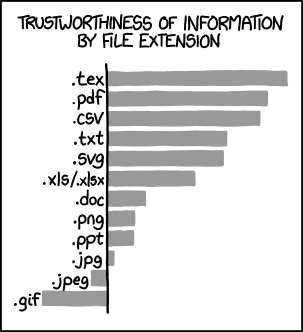
\includegraphics[width=0.5\textwidth]{file_extensions}
	\end{center}
\end{minipage}

Les sources peuvent être de différentes natures :
\begin{itemize}
	\item tutoriel/cours directement accessibles sur sites Webs : dans la \textit{majorité}\footnote{La précision est importante, il y a toujours des exceptions.} des cas, informations assez basiques sur un sujet, peu de détails vraiment pointus.
	\item vidéos YouTube : \textit{idem} que précédemment.
	\item documentations de systèmes ou de bibliothèques (ou de manière équivalente \textit{datasheets}, manuels, \dots) : extrêmement pointus mais aussi très spécifique, ces documents ne servent que dans des cas très particuliers d'applications
	\item livres (format papier ou \textit{PDF}) : objectif exprès de partage de connaissances qui vont souvent de basiques à très pointus.
\end{itemize}
\subsubsection{Sites Webs}
Sources textuelles d'information directe les plus importantes :
\begin{itemize}
	\item Wikimédia :
		\begin{itemize}
			\item Wikilivres : moins large et beaucoup moins pointu dans l'ensemble, propose des cours pour découvrir les bases d'un domaine.
			\item Wikipédia : le classique indémodable, contient selon les sujets des informations parfois très pointus. Très fiable en informatique dans l'ensemble.
		\end{itemize}
	\item Microsoft Doc : documentation et tutoriels très concis sur certains outils en rapport avec Windows (langages C/C++, PowerShell, outils .NET, \dots)
	\item Zeste de Savoir : site de très grande qualité, généraliste au niveau scientifique, dont tous les cours sont relus et validés par les pairs
	\item Developpez.com : site traitant d'informatique proposant des cours écrits par des bénévoles\footnote{La qualité peut varier fortement selon les auteurs.} sur un très large panel de sujets
	\item Os-Dev.org : site sous forme de wiki traitant du sujet spécifique du développement de systèmes d'exploitation
	\item le site du zéro : connaissances de bases sur plusieurs sujets d'informatique
\end{itemize}
\textbf{Remarque : }Openclassroom (nouvelle bouture capitaliste du site du zéro) n'est pas listé car particulièrement pauvre et superficiel dans les connaissances apportées.

Chaînes YouTube\footnote{Y a pas grand-chose parce-que pour trouver autre chose que la vulgarisation ou des trucs bateaux il faut se lever de bonne heure. Peut-être que ça existe, je n'ai juste pas trouvé.} :
\begin{itemize}
	\item \href{https://www.youtube.com/@mitocw}{VOD de cours du MIT} : des cours complets sur un tas de sujets, pas toujours très agréable sur la forme, mais intéressants. \textit{À regarder en x2, a minima x1.5}.
	\item \href{https://www.youtube.com/@cem_yuksel}{Cem Yuksel} : professeur d'informatique graphique en université
	\item \href{https://www.youtube.com/@informatiquetheorique9146}{Informatique théorique} : informatique de classes préparatoires et de master.
	\item \href{https://www.youtube.com/@3blue1brown}{3Blue1Brown} : pour développer son intuition sur un tas de sujets scientifiques (majoritairement mathématiques et informatique)
	\item \href{https://www.youtube.com/@writeyourownoperatingsystem}{Write your own operating system} : chaîne spécialisée dans le développement de systèmes d'exploitation
\end{itemize}
\subsubsection{Documentation en ligne}
\subsubsection{Livres}
Les livres, au format PDF comme papier, forment la base de connaissances la plus complète et la mieux construite que l'on puisse trouver. Pour trouver un livre sur un sujet, le mieux reste de chercher une liste de livres sur un sujet et prendre le premier. Une simple recherche sur Internet du type : \textit{books $<$subject$>$} devrait suffire pour obtenir une liste de livres classiques sur un sujet.

Il y a ensuite deux choix :
\begin{itemize}
	\item trouver le livre papier (en bibliothèque, ou l'acheter)
	\item trouver le livre PDF (en archives ou bibliothèques ou l'acheter)
\end{itemize}
Une grande quantité de PDFs d'excellents livres en informatique peuvent être trouvés sur ce \href{https://drive.google.com/drive/u/1/folders/1fdPcRYRMhrEyqla_tYT2RyoFctbnXPn5}{Google Drive}. Un document d'indication est donné.
\subsubsection{Documentation hors-ligne}
La commande \textit{man} du terminal Linux est probablement la commande la plus utile au développeur C.
\subsection{Lire un prototype}
	Abbréviations classiques : fd, buffer, etc...
\subsection{Liste des sites de forum}
	\subsubsection{Stack Overflow}
	\subsubsection{developpez.com}
\subsection{À propos des GPTs}
\textbf{Avis de l'auteur quant à l'utilisation d'intelligences artificielles de type LLM (\textit{\underline{L}arge \underline{L}anguage \underline{M}odels} en anglais)}\footnote{Personne ne me l'a demandé et je vais probablement passer pour un moralisateur invétéré, mais merde !} :
 
La programmation à l'aide de modèles de langage n'est utile que pour gagner du temps lors de l'écriture de code redondant ou pour l'écriture de documentation (processus en général très peu formateur, redondant et ennuyeux). En effet, l'écriture de ces textes ne demande aucune intelligence et n'apprend rien puisque tout est réfléchi par une intelligence tierce. Cela ne peut être remis en cause à mon avis.
 
Par voie de conséquence, il devient évident que l'utilisation de LLMs pour apprendre à programmer (j'entends par là : écrire à sa place le code\footnote{Et pas demander une explication}) est non seulement inutile mais contre-productif à toute apprentissage, puisque la maîtrise de notions complexes nécessite la maîtrise des fondamentaux, et que rien ne vaut pour véritablement comprendre et assimiler une chose que de la prendre entre quatre yeux et y passer le temps qu'il faut, malgré toute la fatigue que cela peut induire. Dans le cas de projets personnels, il doit être plus épanouissant de réussir à résoudre un problème par soi-même que de copier la solution d'un autre, et c'est de cette façon que non content d'une progression pérenne, le travailleur peut voir en son travail une source de bonheur.\footnote{Aucune influence ici d'un certain programme littéraire de classe préparatoire 2023, c'est évident `,-D}
 
Par ailleurs, les LLMs ont une tendance certaine à moyenner. Cela signifie en particulier que rien de particulièrement excellent ne sortira, sauf coup de chance extraordinaire, d'un GPT classique\footnote{Il ne faut extrapoler à toutes les intelligences artificielles. Il s'agirait là d'une bien mauvaise généralisation. Le programme \textit{Alpha Dev} de DeepMind a pu améliorer certains algorithmes classiques au delà de ce qui était humainement connu à ce moment. Il s'agit toutefois d'une IA spécialisée.}. Les codes générés ne seront donc pas extraordinaires et pourront servir à un apprentissage de qualité.

Quant à l'utilité de cet outil pour des problèmes :
\begin{enumerate}
\item dont la résolution sera \textit{évaluée} de quelque manière que ce soit par une partie d'un corps enseignant
\item devant être fait dans le cadre d'un travail professionnel dans un temps très court et/ou dans un pur but de productivité
\item pour toute autre raison pour laquelle l'apprentissage et la réflexion ne sont pas exigés, et sur un sujet pour lequel le développeur n'éprouve strictement aucun intérêt
\end{enumerate}
, l'auteur :
\begin{enumerate}
\item jugeant le système construit autour de la notation particulièrement désuet et dépourvu d'attraits pédagogiques\footnote{Si tant est que l'on puisse être ``pédagogique'' à forcer un élève dans un enseignement sans jamais tenter de l'intéresser autrement que par le désir d'un nombre plus ou moins élevé qui ne reflétera que très peu son intelligence ou son investissement. Enfin quoi ! Il doit y avoir d'autres moyens d'accrocher les étudiants aux cours, non ?}
\item se trouvant être marxiste\footnote{plutôt marxien pour ceux qui apprécient les nuances} et donc convaincu de la nécessité de l'épanouissement humaoin
\item n'appréciant pas de se faire chier pour \textit{aucune} raison
\end{enumerate}
ne voit aucun mal à ChatGPT pour ce qui est de répondre aux exigences d'entités soit incompétentes\footnote{Aucun rapport avec certains charlatans dont les existences ont conduit à l'écriture de ce livre. Évidemment\dots} soit n'ayant aucune considération pour l'étudiant/le travailleur.


\end{document}